\section{一阶线性方程}
\label{sec:lde-first-order}

最简单的线性方程只有一个未知函数和一阶导数。设$I$是一个区间，$a,g:I\to\mathbb{R}$是给定函数，考虑
\begin{equation}
 \dot{x}(t)=a(t)x(t)+g(t),\qquad x(t_0)=x_0,\qquad t_0\in I.
 \label{eq:lde-scalar}
\end{equation}
称它为\term{一阶线性方程}（first-order linear equation）。系数$a(t)$说明当前状态怎样影响自身的变化，$g(t)$是外部输入。$g\equiv0$时方程称为\term{齐次线性方程}（homogeneous linear equation），否则称为非齐次线性方程。

\paragraph{叠加}
线性的含义可以直接验证。若$x_1$满足$\dot{x}_1=ax_1+g_1$，$x_2$满足$\dot{x}_2=ax_2+g_2$，则对常数$c_1,c_2$，组合$c_1x_1+c_2x_2$满足同一个方程，输入变为$c_1g_1+c_2g_2$。这就是\term{叠加原理}（superposition principle）。

特别地，同一输入下两个解的差满足齐次方程。所以只要找到一个解，其他解都等于它加上某个齐次解。下面的工作因此分成两件事：求齐次解，求一个带输入的解。

\paragraph{从乘积求导到积分因子}
方程~\eqref{eq:lde-scalar}的困难在于$\dot{x}-ax$不是任何函数的导数，无法直接积分。乘积求导公式却提供了一种可能。对一个待定的正函数$\mu(t)$，有
\[
 \frac{\mathrm{d}}{\mathrm{d}t}\bigl(\mu x\bigr)=\mu\dot{x}+\dot{\mu}x.
\]
把方程改写成$\dot{x}-ax=g$，两边乘$\mu$，左边是$\mu\dot{x}-a\mu x$。只要它恰好是上面的乘积导数，就要求
\[
 \dot{\mu}=-a\mu.
\]

这是一个不含$x$的齐次方程，它的一个正解是
\begin{equation}
 \mu(t)=\exp\Bigl(-\int_{t_0}^{t}a(r)\,\mathrm{d}r\Bigr).
 \label{eq:lde-integrating-factor}
\end{equation}
这个$\mu$称为\term{积分因子}（integrating factor），选取下限$t_0$使$\mu(t_0)=1$。乘上它之后，方程变成
\[
 \frac{\mathrm{d}}{\mathrm{d}t}\bigl(\mu(t)x(t)\bigr)=\mu(t)g(t).
\]

右端不再含未知函数，从$t_0$积分到$t$，并利用$\mu(t_0)=1$，得到
\[
 \mu(t)x(t)-x_0=\int_{t_0}^{t}\mu(s)g(s)\,\mathrm{d}s.
\]
两边除以$\mu(t)$就解出了$x(t)$。比值$\mu(s)/\mu(t)$恰好等于从$s$到$t$累积系数的指数，记
\begin{equation}
 \Phi(t,s)=\frac{\mu(s)}{\mu(t)}=\exp\Bigl(\int_{s}^{t}a(r)\,\mathrm{d}r\Bigr).
 \label{eq:lde-scalar-propagator}
\end{equation}
$\Phi(t,s)$把时刻$s$的齐次状态传播到时刻$t$，第~\ref{sec:lde-time-varying}节会建立它的矩阵版本。

\begin{theorem}[连续系数的一阶线性方程]
\label{thm:lde-scalar-solution}
设$a,g$在区间$I$上连续，$t_0\in I$，$x_0\in\mathbb{R}$。则初值问题~\eqref{eq:lde-scalar}在整个$I$上有唯一的连续可微解，它是
\begin{equation}
 x(t)=\Phi(t,t_0)x_0+\int_{t_0}^{t}\Phi(t,s)g(s)\,\mathrm{d}s.
 \label{eq:lde-scalar-solution}
\end{equation}
\end{theorem}

\begin{proof}
先证唯一。设$x$是$I$上的连续可微解，上面的推导每一步都合法：$\mu$连续可微且恒正，乘积求导成立，$\mu g$连续，可以用微积分基本定理积分。所以$x$必须等于式~\eqref{eq:lde-scalar-solution}。

再证这个公式确实给出解。由式~\eqref{eq:lde-scalar-propagator}，它可以写成
\[
 x(t)=\frac{1}{\mu(t)}\Bigl(x_0+\int_{t_0}^{t}\mu(s)g(s)\,\mathrm{d}s\Bigr).
\]
由$\dot{\mu}=-a\mu$得$(1/\mu)^{\cdot}=a/\mu$。对乘积求导，第一项得$a(t)x(t)$，第二项由积分上限求导得$g(t)$，所以
\[
 \dot{x}(t)=a(t)x(t)+g(t).
\]
代入$t=t_0$，积分为零，$\Phi(t_0,t_0)=1$，得$x(t_0)=x_0$。
\end{proof}

公式~\eqref{eq:lde-scalar-solution}的两项有清楚的含义。第一项是初值独自传播的结果。第二项把每一时刻的输入$g(s)\,\mathrm{d}s$看成一笔小的状态增量，它从时刻$s$起按$\Phi(t,s)$传播到$t$，再全部累加。

连续性条件的作用也很具体：它保证$\mu$可微，保证$\mu g$能用微积分基本定理积分。结论中的存在区间是整个$I$，这与非线性方程不同。第~\ref{chap:ordinary-differential-equations}章的$\dot{x}=x^2$、$x(0)=1$有解$1/(1-t)$，在$t=1$爆炸；线性方程右端关于$x$只按一次增长，公式~\eqref{eq:lde-scalar-solution}在系数有定义的地方都有意义。

\begin{example}[正弦输入的散热]
\label{ex:lde-sine-input}
求解$\dot{x}=-x+\sin t$，$x(0)=x_0$。这里$a=-1$，所以$\Phi(t,s)=\mathrm{e}^{-(t-s)}$。由式~\eqref{eq:lde-scalar-solution}，
\[
 x(t)=\mathrm{e}^{-t}x_0+\mathrm{e}^{-t}\int_0^t\mathrm{e}^{s}\sin s\,\mathrm{d}s.
\]
分部积分两次可得$\mathrm{e}^{s}(\sin s-\cos s)/2$是$\mathrm{e}^{s}\sin s$的一个原函数，于是
\[
 \int_0^t\mathrm{e}^{s}\sin s\,\mathrm{d}s=\frac{\mathrm{e}^{t}(\sin t-\cos t)+1}{2}.
\]
代回并合并$\mathrm{e}^{-t}$的项，得到
\[
 x(t)=\Bigl(x_0+\frac12\Bigr)\mathrm{e}^{-t}+\frac{\sin t-\cos t}{2}.
\]
令$x_{\mathrm{p}}(t)=(\sin t-\cos t)/2$，它是$x_0=-1/2$对应的特解。对它求导，
\[
 \dot{x}_{\mathrm{p}}=\frac{\cos t+\sin t}{2}=-x_{\mathrm{p}}+\sin t,
\]
所以$x_{\mathrm{p}}$确实满足方程。常数$x_0+1/2$由初值唯一确定。
\end{example}

图~\ref{fig:lde-first-order-family}把这个分解画了出来。方向场的短线段是每点的斜率，解曲线沿短线段前进。不同初值的解之差是$(x_0-x_0')\mathrm{e}^{-t}$，它们在几个时间单位内贴到同一条黄色曲线上。

\begin{BookInlineFigure}
  \centering
  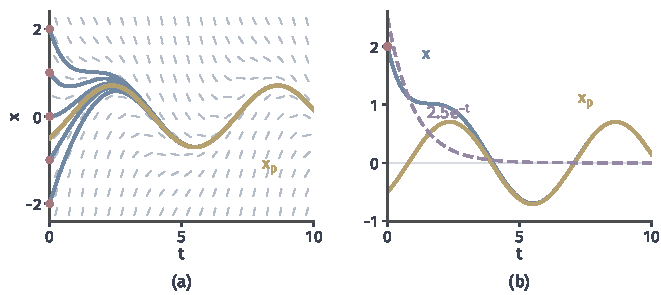
\includegraphics[width=112mm]{figures/06-differential-equations/01-ordinary-differential-equations/matplotlib/lde-first-order-family/figure.pdf}
  \caption{方程$\dot{x}=-x+\sin t$的解族与分解。(a)灰色短线是方向场，蓝线是初值$x_0=-2,-1,0,1,2$（红点）的解，黄线是特解$x_{\mathrm{p}}$。(b)$x_0=2$的解（蓝）等于紫色虚线$2.5\mathrm{e}^{-t}$与黄色特解之和。}
  \label{fig:lde-first-order-family}
\end{BookInlineFigure}

\paragraph{积分因子做了什么}
再看一个系数随时间变化的例子，$\dot{x}=-2tx+2t$，$x(0)=x_0$。这里$\int_0^t a=-t^2$，积分因子是$\mu(t)=\mathrm{e}^{t^2}$。令$y=\mu x$，方程变成
\[
 \dot{y}=2t\mathrm{e}^{t^2}.
\]
右端不再依赖状态，积分得到$y(t)=x_0+\mathrm{e}^{t^2}-1$。除以$\mu$，结果是
\[
 x(t)=1+(x_0-1)\mathrm{e}^{-t^2}.
\]

图~\ref{fig:lde-integrating-factor}对比了$x$和$y$两个坐标。原坐标中的解曲线互相靠拢，斜率同时依赖$t$和$x$。换成$y=\mu x$以后，同一时刻各点斜率相同，解曲线彼此只差一个上下平移，积分因此可以直接进行。

可以把$\mu(t)$想成一把随时间伸缩的尺子。齐次部分造成的伸缩被这把尺子抵消，剩下的只有输入的累积。这个类比只对线性方程成立：非线性方程中伸缩率依赖状态本身，不同解需要不同的尺子。

\begin{BookInlineFigure}
  \centering
  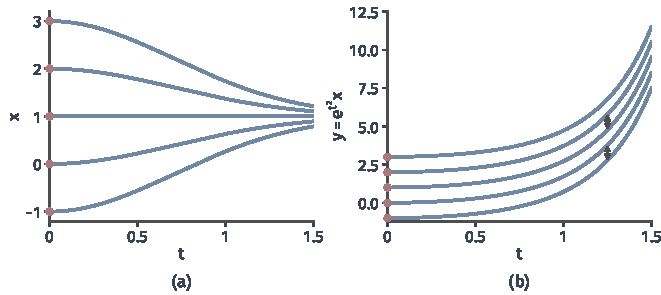
\includegraphics[width=112mm]{figures/06-differential-equations/01-ordinary-differential-equations/matplotlib/lde-integrating-factor/figure.pdf}
  \caption{积分因子的作用，方程$\dot{x}=-2tx+2t$，红点是初值$x_0=-1,0,1,2,3$。(a)原坐标中的解。(b)变量$y=\mathrm{e}^{t^2}x$下，同一批解彼此只差上下平移，黑色双箭头示意相邻两条曲线在同一时刻的间距都是$1$。}
  \label{fig:lde-integrating-factor}
\end{BookInlineFigure}

\paragraph{解的区间由系数决定}
定理~\ref{thm:lde-scalar-solution}要求系数在$I$上连续，$I$之外不作任何保证。考虑$\dot{x}=-x/t+1$，$x(1)=x_0$。系数$a(t)=-1/t$在$t=0$没有定义，初值点$t_0=1$所在的最大连续区间是$I=(0,\infty)$。

由式~\eqref{eq:lde-scalar-propagator}，$\Phi(t,s)=\exp(-\ln t+\ln s)=s/t$。代入式~\eqref{eq:lde-scalar-solution}，
\[
 x(t)=\frac{x_0}{t}+\int_1^t\frac{s}{t}\,\mathrm{d}s=\frac{x_0}{t}+\frac{t^2-1}{2t}.
\]
令$c=x_0-1/2$，解化成
\[
 x(t)=\frac{c}{t}+\frac{t}{2},\qquad t\in(0,\infty).
\]

图~\ref{fig:lde-singular-coefficient}中，$c\neq0$的解在$t\to0^+$时无界，$c=0$的解$x=t/2$却可以一直延伸到$t=0$。这里的奇异位置$t=0$由系数决定，所有解都在同一处遇到它；而$\dot{x}=x^2$的爆炸时刻随初值变化。线性方程的解走不出系数的连续区间，也只有在这个边界上才可能失控。

\begin{BookInlineFigure}
  \centering
  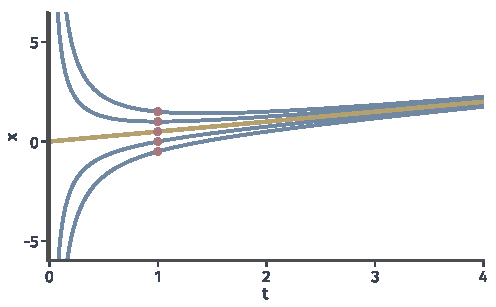
\includegraphics[width=84mm]{figures/06-differential-equations/01-ordinary-differential-equations/matplotlib/lde-singular-coefficient/figure.pdf}
  \caption{系数决定解的区间。方程$\dot{x}=-x/t+1$的解$x=c/t+t/2$，红点是$t=1$处的初值，蓝线取$c=\pm1,\pm0.5$，黄线取$c=0$。左侧深灰粗线$t=0$处系数$-1/t$无定义，所有$c\neq0$的解都在此无界。}
  \label{fig:lde-singular-coefficient}
\end{BookInlineFigure}

\paragraph{可积系数}
第~\ref{chap:ordinary-differential-equations}章说明过，系数或输入只是可测时，解未必处处可微，要用积分形式理解。对线性方程，这种解的含义是：$x$在$I$的每个紧子区间上绝对连续，在$I$上几乎处处满足微分方程，并且$x(t_0)=x_0$。与之等价的写法是
\begin{equation}
 x(t)=x_0+\int_{t_0}^{t}\bigl(a(s)x(s)+g(s)\bigr)\,\mathrm{d}s,\qquad t\in I.
 \label{eq:lde-scalar-integral}
\end{equation}
绝对连续函数的导数几乎处处存在且可积，并能积分回原函数，可参考\BookChapterRef{chap:integration}{卷四第6章“积分”}。

\begin{theorem}[可积系数的一阶线性方程]
\label{thm:lde-scalar-integrable}
设$a,g$在$I$的每个紧子区间上Lebesgue可积，$t_0\in I$。则式~\eqref{eq:lde-scalar-solution}定义的函数是积分方程~\eqref{eq:lde-scalar-integral}在$I$上的唯一局部绝对连续解。
\end{theorem}

\begin{proof}
此时$b(t)=\int_{t_0}^ta$局部绝对连续，$\mu=\mathrm{e}^{-b}$是绝对连续函数与光滑函数的复合，在紧子区间上$b$有界，所以$\mu$与$1/\mu$都局部绝对连续，并且几乎处处有$\dot{\mu}=-a\mu$。

先证唯一。设$x$是局部绝对连续解。局部绝对连续函数的乘积仍局部绝对连续，所以$\mu x$局部绝对连续，几乎处处有
\[
 (\mu x)^{\cdot}=\mu(\dot{x}-ax)=\mu g.
\]
$\mu$在紧子区间上有界，$\mu g$可积。对绝对连续函数用微积分基本定理，得$\mu(t)x(t)-x_0=\int_{t_0}^t\mu g$，这正是式~\eqref{eq:lde-scalar-solution}。

再证存在。令$y(t)=x_0+\int_{t_0}^t\mu g$，它局部绝对连续，几乎处处$\dot{y}=\mu g$。令$x=y/\mu$，它局部绝对连续，并且几乎处处
\[
 \dot{x}=\frac{a}{\mu}y+\frac{1}{\mu}\mu g=ax+g.
\]
再积分回去就得到式~\eqref{eq:lde-scalar-integral}。
\end{proof}

公式没有变化，变化的只是它的解释：求导只在几乎处处成立，真正对每一点都成立的是积分形式。图~\ref{fig:lde-integrable-coefficient}给出两种典型情况。

\begin{example}[两种不光滑的系数]
\label{ex:lde-integrable-coefficients}
第一种是系数跳变。取$x(0)=1$，$g=0$，$a(t)=-1$（$0\leq t<1$），$a(t)=-3$（$t\geq1$）。计算$\int_0^t a$，得到
\[
 x(t)=\begin{cases}\mathrm{e}^{-t},&0\leq t\leq1,\\ \mathrm{e}^{-1}\mathrm{e}^{-3(t-1)},&t\geq1.\end{cases}
\]
左导数$-\mathrm{e}^{-1}$与右导数$-3\mathrm{e}^{-1}$在$t=1$不同，解在这一点不可微，其余各点都满足方程。

第二种是系数在端点无界但可积。取$a(t)=-1/(2\sqrt{t})$，$x(0)=1$。由$\int_0^ta=-\sqrt{t}$得
\[
 x(t)=\mathrm{e}^{-\sqrt{t}}.
\]
它在$t>0$满足方程，导数$-\mathrm{e}^{-\sqrt{t}}/(2\sqrt{t})$在$t\to0^+$时趋于$-\infty$。$x$在$t=0$不可微，式~\eqref{eq:lde-scalar-integral}仍然成立。
\end{example}

\begin{BookInlineFigure}
  \centering
  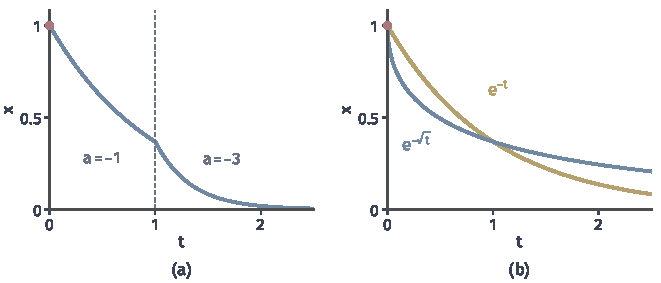
\includegraphics[width=112mm]{figures/06-differential-equations/01-ordinary-differential-equations/matplotlib/lde-integrable-coefficient/figure.pdf}
  \caption{可积系数下的绝对连续解，红点是初值$x(0)=1$。(a)系数在$t=1$从$-1$跳到$-3$，解连续但有折角。(b)系数$-1/(2\sqrt{t})$在$0$处无界但可积，解$\mathrm{e}^{-\sqrt{t}}$（蓝）在$0$处切线竖直；黄线$\mathrm{e}^{-t}$作对照，它在$0$处斜率有限。}
  \label{fig:lde-integrable-coefficient}
\end{BookInlineFigure}
